%!TEX root = ../fbi.tex

\section{Quasi-local parent Hamiltonian and perturbations}
\label{sec:perturbations}

In this section we strive to confirm the claims of Section~\ref{sec:symmetry} about
which perturbations split the entanglement degeneracy of the odd size cylinders.

This could be achieved for example by adding a staggered field 
$$
H' = h \sum\limits_{i} (-1)^i \left(b_i + b_i^{\dagger}\right),
$$
where the coefficients $(-1)^i$ takes opposite values on the two sublattices, 
to a Hamiltonian for the state. More complicated staggering fields that break translational 
symmetry but change sign under inversion can be also be used - additionally, the symmetry $\I_y$ 
can be used in place of $\I$ which protects against different sets of patterns of staggering the 
field.

\begin{figure}[htbp]
	\centering
		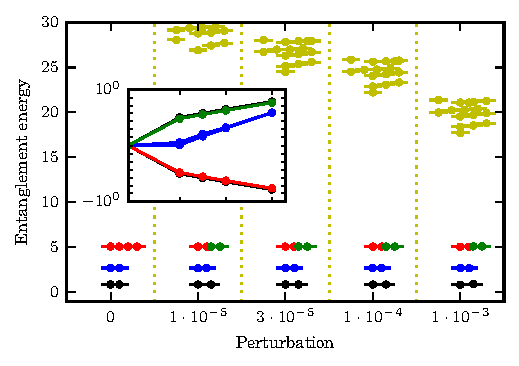
\includegraphics[width=\columnwidth]{symbreaking_EE.pdf}
	\caption{Entanglement spectrum under symmetry breaking perturbations}
	\label{fig:symbreaking_EE}
\end{figure}

\begin{figure}[htbp]
	\centering
		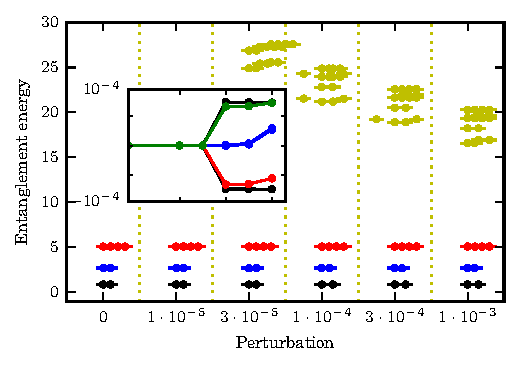
\includegraphics[width=\columnwidth]{sympreserving_EE.pdf}
	\caption{Entanglement spectrum under symmetry preserving perturbations}
	\label{fig:symbreaking_EE}
\end{figure}


\section{String Order Parameter}
\label{sec:stringorder}
?


